\documentclass[11pt,a4paper]{article}

% Packages
\usepackage[utf8]{inputenc}
\usepackage[T1]{fontenc}
\usepackage{amsmath,amssymb,amsthm}
\usepackage{graphicx}
\usepackage{hyperref}
\hypersetup{colorlinks=true,citecolor=blue,linkcolor=blue,urlcolor=blue}
\usepackage{booktabs}
\usepackage{natbib}
\usepackage[margin=1in]{geometry}
\usepackage{algorithm}
\usepackage{algpseudocode}
\usepackage{subcaption}

% Theorem environments
\newtheorem{definition}{Definition}
\newtheorem{proposition}{Proposition}

\title{Topological Binding Detection in Coupled Dynamical Systems\\via Persistent Homology}
\author{ATT Contributors}
\date{March 2026}

\begin{document}
\maketitle

\begin{abstract}
We introduce a method for detecting emergent topological structure in coupled dynamical systems using persistent homology on delay embeddings.
Given two coupled time series, we construct Takens delay embeddings of each marginal system and of the joint system, compute persistence images on all three point clouds using a shared grid, and identify excess homology in the joint embedding that is absent from both marginals.
This \emph{topological binding score} quantifies coupling-induced geometric structure that information-theoretic and recurrence-based measures cannot capture.
We validate the method on coupled Lorenz and R\"ossler--Lorenz systems, demonstrating: (i) a coupling-dependent binding response that rises from baseline at low coupling and collapses at synchronization; (ii) surrogate-tested significance with controlled false positive rates; (iii) robustness to heterogeneous intrinsic timescales via per-channel delay estimation; (iv) greater sensitivity to coupling than transfer entropy, phase-amplitude coupling, and cross-recurrence quantification in a head-to-head benchmark; (v) sliding-window topological transition detection on synthetic bistable EEG, identifying regime changes between oscillatory states; (vi) real EEG validation on binocular rivalry SSVEP data \citep{nie2023accumulating} across $N = 80$ subjects, where the detector achieves $94.1\%$ mean precision at 5\,s tolerance (median 100\%, 80\% of subjects with zero false alarms) and $40.6\%$ mean recall, capturing major perceptual switches as topological reorganizations; (vii) cross-region binding analysis on occipital--parietal EEG channels, where joint topology of Oz--Pz embeddings reveals coupling that modulates with perceptual instability (single-subject: Spearman $\rho = 0.51$, $p = 0.016$);
(viii) multi-subject cross-region binding ($N = 79$), where the population mean binding--switch correlation is significantly positive (mean $\rho = 0.10$, $t_{78} = 3.35$, $p = 0.001$; Wilcoxon $p = 0.001$; 60.8\% of subjects showing positive correlations, binomial $p = 0.036$), confirming that occipital--parietal topological coupling modulates with perceptual state at the population level;
and (ix) z-score calibration against surrogate null distributions, revealing that the method is selectively sensitive to heterogeneous-timescale coupling (R\"ossler--Lorenz: 3/5 seeds significant at $p \leq 0.05$) while having zero power for same-timescale coupling (Lorenz--Lorenz: all z-scores negative).
The method is implemented in the open-source \texttt{att-toolkit} Python package.
\end{abstract}

\section{Introduction}

Detecting and characterizing coupling between dynamical systems is a central problem in nonlinear time series analysis, with applications ranging from climate science \citep{schreiber2000measuring} to neuroscience \citep{fries2005mechanism}.
Existing methods quantify coupling through information transfer (transfer entropy), cross-frequency interactions (phase-amplitude coupling (PAC) \citep{tort2010measuring}), or shared recurrence structure (cross-recurrence quantification analysis (CRQA) \citep{marwan2007recurrence}).
While effective in their respective domains, these methods do not capture the \emph{geometry} of coupling --- the topological structure that emerges in the joint state space when two systems interact.

Topological data analysis (TDA), particularly persistent homology \citep{carlsson2009topology, edelsbrunner2010computational}, provides tools for characterizing the shape of point clouds at multiple scales.
Applied to delay-embedded time series, persistent homology recovers topological invariants of the underlying attractor \citep{perea2015sliding}.
However, existing TDA approaches to coupling analysis operate in derived spaces (e.g., correlation matrices \citep{giusti2015clique}, transfer entropy networks \citep{xi2023directed}) rather than directly in the reconstructed state space.

We propose a direct approach: compare the persistent homology of the joint delay embedding against the persistent homology of each marginal delay embedding.
Topological features present in the joint but absent from both marginals constitute \emph{topological binding} --- emergent geometric structure created by the coupling.
This construction exploits Takens' embedding theorem \citep{takens1981detecting, sauer1991embedology}, which guarantees that delay embeddings of coupled systems with sufficient dimension recover the topology of the coupled attractor.

The key technical contributions are:
\begin{enumerate}
    \item \textbf{Joint-vs-marginal persistent homology}: A construction that identifies excess homology classes in joint Takens embeddings relative to marginal embeddings (Section~\ref{sec:method}).
    \item \textbf{Persistence image subtraction with configurable baselines}: A practical implementation using vectorized persistence representations with explicit design justification for the baseline choice (Section~\ref{sec:binding}).
    \item \textbf{Embedding quality gating}: An automated degeneracy check that prevents topological artifacts from contaminating binding scores (Section~\ref{sec:quality}).
    \item \textbf{Surrogate-tested significance}: A statistical framework using amplitude-adjusted Fourier transform surrogates for hypothesis testing (Section~\ref{sec:significance}).
    \item \textbf{Head-to-head benchmarks}: The first published comparison of a TDA-based coupling measure against TE, PAC, and CRQA on identical coupled chaotic systems with explicit normalization (Section~\ref{sec:exp-benchmarks}).
    \item \textbf{Sliding-window transition detection}: A method for detecting topological regime changes in time series via persistence image distances and CUSUM changepoint detection (Section~\ref{sec:res-transitions}).
    \item \textbf{Real EEG validation}: The first application of sliding-window persistent homology to real binocular rivalry EEG, demonstrating 100\% precision in detecting perceptual switches as topological changepoints (Section~\ref{sec:res-real-eeg}).
    \item \textbf{Cross-region binding}: The first application of joint-vs-marginal persistent homology to multi-channel EEG, quantifying occipital--parietal topological coupling and its modulation by perceptual instability (Section~\ref{sec:res-cross-binding}).
    \item \textbf{Domain of applicability}: Identification of the method's operating regime via z-score calibration --- selective sensitivity to heterogeneous-timescale coupling, zero power for same-timescale coupling, and honest characterization of score variability and N-body contamination (Section~\ref{sec:res-zscore}).
\end{enumerate}


\section{Background}

\subsection{Attractor Reconstruction}

Takens' embedding theorem \citep{takens1981detecting} establishes that for a generic smooth dynamical system with attractor of box-counting dimension $d_A$, the time-delay embedding
\begin{equation}
    \mathbf{x}(t) = \bigl(x(t),\, x(t-\tau),\, x(t-2\tau),\, \ldots,\, x(t-(m-1)\tau)\bigr) \in \mathbb{R}^m
\end{equation}
with embedding dimension $m \geq 2d_A + 1$ produces a diffeomorphic copy of the original attractor from a single scalar observation $x(t)$.
The delay $\tau$ is typically estimated via the first minimum of average mutual information (AMI) \citep{fraser1986independent}, and the dimension $m$ via the false nearest neighbors (FNN) criterion \citep{kennel1992determining}.

For two coupled systems observed via $h_1: M_1 \to \mathbb{R}$ and $h_2: M_2 \to \mathbb{R}$, the \emph{joint delay embedding} concatenates delay vectors from both observations:
\begin{equation}
    \mathbf{z}(t) = \bigl(x(t), \ldots, x(t-(m_1-1)\tau_1),\; y(t), \ldots, y(t-(m_2-1)\tau_2)\bigr) \in \mathbb{R}^{m_1+m_2}
\end{equation}
where $(\tau_1, m_1)$ and $(\tau_2, m_2)$ are estimated independently for each channel.
When the coupled attractor $A \subset M_1 \times M_2$ is not a product $A_1 \times A_2$, the joint embedding captures topological structure inaccessible to either marginal embedding alone.

\subsection{Persistent Homology}

Given a point cloud $P \subset \mathbb{R}^D$, persistent homology tracks the evolution of homological features (connected components $H_0$, loops $H_1$, voids $H_2$, etc.) across the Vietoris--Rips filtration parameterized by scale $\epsilon$ \citep{edelsbrunner2010computational}.
Each feature has a birth time $b$ and death time $d$; long-lived features ($d - b$ large) represent robust topological structure.

\textbf{Persistence images} \citep{adams2017persistence} provide a stable, vectorized representation by placing a weighted Gaussian at each point $(b, d-b)$ in birth--persistence coordinates, then evaluating on a grid.
Crucially, persistence images support linear operations: subtraction, averaging, and inner products are well-defined.
This makes them suitable for our binding detection framework, where the core operation is subtracting marginal persistence images from the joint persistence image.


\section{Method}\label{sec:method}

\subsection{Binding Detection via Persistence Image Subtraction}\label{sec:binding}

Given coupled time series $X = \{x(t)\}$ and $Y = \{y(t)\}$:

\begin{enumerate}
    \item \textbf{Marginal embeddings}: Construct delay embeddings $\mathcal{C}_X$ and $\mathcal{C}_Y$ using per-channel AMI/FNN estimation.
    \item \textbf{Joint embedding}: Construct $\mathcal{C}_{XY}$ using independently estimated delays and dimensions for each channel.
    \item \textbf{Quality gate}: Validate all three embeddings via singular value decomposition (Section~\ref{sec:quality}).
    \item \textbf{Persistence computation}: Compute Vietoris--Rips persistence diagrams $\text{Dgm}_d(\mathcal{C})$ for $d \in \{0, 1\}$ on each point cloud, using identical subsampling seeds.
    \item \textbf{Shared grid alignment}: Compute the union of birth and persistence ranges across all three diagram sets. Evaluate all persistence images on this shared grid.
    \item \textbf{Residual computation}: For each homology dimension $d$,
    \begin{equation}\label{eq:residual}
        R_d = I_d^{XY} - B_d(I_d^X, I_d^Y)
    \end{equation}
    where $I_d^{(\cdot)}$ denotes the persistence image and $B_d$ is the baseline function.
    \item \textbf{Binding score}: $S = \sum_d \| \max(R_d, 0) \|_1$, the $L^1$ norm of the positive part of the residual summed across dimensions.
\end{enumerate}

\begin{algorithm}
\caption{Binding Detection}
\label{alg:binding}
\begin{algorithmic}[1]
\Require Time series $X$, $Y$; max homology dimension $D$; baseline type $B$
\Ensure Binding score $S$, residual images $\{R_d\}_{d=0}^D$
\State $\mathcal{C}_X \gets \Call{TakensEmbed}{X, \tau_X^*, m_X^*}$ \Comment{Auto delay/dim}
\State $\mathcal{C}_Y \gets \Call{TakensEmbed}{Y, \tau_Y^*, m_Y^*}$
\State $\mathcal{C}_{XY} \gets \Call{JointEmbed}{X, Y, [\tau_X^*, \tau_Y^*], [m_X^*, m_Y^*]}$
\State \Call{ValidateEmbedding}{$\mathcal{C}_X, \mathcal{C}_Y, \mathcal{C}_{XY}$} \Comment{Quality gate}
\For{$\mathcal{C} \in \{\mathcal{C}_X, \mathcal{C}_Y, \mathcal{C}_{XY}\}$}
    \State Compute $\text{Dgm}_d(\mathcal{C})$ for $d = 0, \ldots, D$ via Ripser \citep{bauer2021ripser}
\EndFor
\State Compute shared birth/persistence ranges from all diagrams
\For{$d = 0, \ldots, D$}
    \State $I_d^X, I_d^Y, I_d^{XY} \gets$ persistence images on shared grid
    \If{$B = \text{max}$}
        \State $R_d \gets I_d^{XY} - \max(I_d^X, I_d^Y)$ \Comment{Pointwise max}
    \Else
        \State $R_d \gets I_d^{XY} - (I_d^X + I_d^Y)$ \Comment{Pointwise sum}
    \EndIf
\EndFor
\State $S \gets \sum_{d=0}^{D} \|\max(R_d, 0)\|_1$
\end{algorithmic}
\end{algorithm}

\subsection{Baseline Choice}\label{sec:baseline}

The baseline function $B_d$ in Eq.~\eqref{eq:residual} determines how marginal topologies are combined for comparison against the joint.
We consider two options:

\textbf{Max baseline} (default): $B_d^{\max}(I_d^X, I_d^Y) = \max(I_d^X, I_d^Y)$ pointwise.
A pixel in the residual is positive only if the joint exceeds the \emph{stronger} marginal at that location.
This is conservative: it minimizes false positives because any feature already present in either marginal is not counted as emergent.

\textbf{Sum baseline}: $B_d^{\text{sum}}(I_d^X, I_d^Y) = I_d^X + I_d^Y$.
A pixel is positive only if the joint exceeds the \emph{combined} marginal mass.
This is more sensitive to weak coupling but has a systematic bias: for independent systems, the persistence image of the joint is generally not equal to the sum of marginal persistence images, leading to elevated false positive rates.

We recommend the max baseline for confirmatory analysis and provide the sum baseline as an exploratory alternative.
Both are evaluated in Section~\ref{sec:exp-baseline}.

\subsection{Embedding Quality Gate}\label{sec:quality}

A degenerate joint embedding --- arising, e.g., from a shared delay applied to systems with different intrinsic timescales --- can produce spurious topological features that inflate the binding score.
We validate each embedding via the condition number $\kappa = \sigma_{\max}/\sigma_{\min}$ of the centered point cloud matrix.
If $\kappa > 10^4$ for any of the three embeddings, a warning is issued.
This threshold was calibrated on coupled R\"ossler--Lorenz systems, where per-channel delays produce $\kappa \in [10, 500]$ and shared delays produce $\kappa \in [10^4, 10^8]$.

\textbf{Auto-with-fallback strategy.}
The \texttt{embed\_channel()} function implements a three-stage embedding strategy.
First, AMI and FNN auto-estimation are attempted to determine per-channel delay $\tau$ and embedding dimension $m$.
Second, the resulting embedding is validated via the condition-number check described above.
If the auto-estimated embedding is degenerate ($\kappa > 10^4$) or if auto-estimation fails (e.g., AMI has no local minimum), the method falls back to literature-grounded default parameters: band-specific delays and dimensions derived from \citet{stam2005nonlinear}, which provides empirically validated embedding parameters for common EEG frequency bands.
This fallback ensures that the pipeline produces a usable embedding even when automated parameter selection is unreliable.

\subsection{Significance Testing via Surrogates}\label{sec:significance}

To test the null hypothesis $H_0$: ``the observed binding score is consistent with independent dynamics,'' we use amplitude-adjusted Fourier transform (AAFT) surrogates \citep{schreiber1996improved}.
AAFT surrogates preserve the marginal distribution and power spectrum of $Y$ while destroying coupling to $X$.

For each of $N_s$ surrogates $\tilde{Y}_i$:
\begin{enumerate}
    \item Generate $\tilde{Y}_i$ via AAFT phase randomization of $Y$.
    \item Compute the binding score $\tilde{S}_i$ using $X$ and $\tilde{Y}_i$.
    \item Reuse cached marginal $X$ persistence images (unchanged across surrogates) for efficiency.
\end{enumerate}

The $p$-value is:
\begin{equation}
    p = \frac{1 + \sum_{i=1}^{N_s} \mathbf{1}[\tilde{S}_i \geq S_{\text{obs}}]}{N_s + 1}
\end{equation}

\textbf{Alternative surrogate methods.}
In addition to AAFT, we implement \emph{twin surrogates} \citep{thiel2006twin}, which construct surrogates from the recurrence structure of the embedded attractor itself.
Twin surrogates preserve each system's attractor geometry while destroying inter-system coupling, thereby testing specifically for deterministic nonlinear coupling.
This complements AAFT, which preserves the power spectrum but not the attractor structure.
The choice of surrogate method determines the null hypothesis: AAFT tests against ``coupling beyond what shared spectral structure explains,'' while twin surrogates test against ``coupling beyond what individual attractor dynamics explain.''


\section{Experiments}

\subsection{Experiment 1: Coupling Sweep}\label{sec:exp-sweep}

We sweep the coupling parameter $\epsilon \in [0, 1]$ for two diffusively coupled Lorenz systems:
\begin{align}
    \dot{x}_1 &= \sigma(y_1 - x_1) + \epsilon(x_2 - x_1) \\
    \dot{y}_1 &= x_1(\rho - z_1) - y_1 \\
    \dot{z}_1 &= x_1 y_1 - \beta z_1
\end{align}
with symmetric coupling on $x_2$.
Standard parameters: $\sigma = 10$, $\rho = 28$, $\beta = 8/3$.
Integration via RK45 with $dt = 0.01$, $n = 8000$ steps, 1000-step transient discarded.
Persistence computed on 500-point subsamples with $H_0$ and $H_1$.

\textbf{Expected result}: The binding score should exhibit a coupling-dependent response --- rising at low coupling (emergent joint topology) and declining toward $\epsilon = 1$ as the system approaches complete synchronization and the joint attractor degenerates.
A non-zero baseline at $\epsilon = 0$ is expected because the joint persistence image of independent systems is not identically zero under the max baseline.

\textbf{Figure 1}: Binding score vs.\ coupling strength, with per-dimension ($H_0$, $H_1$) breakdown.

\subsection{Experiment 2: Baseline Comparison}\label{sec:exp-baseline}

Using the same coupled Lorenz sweep, we compare the max and sum baselines across the full coupling range.

\textbf{Expected result}: Both baselines should track coupling monotonically in the low-to-moderate range.
The sum baseline should show higher absolute scores but also elevated values at $\epsilon = 0$ (systematic bias).
The max baseline should have cleaner separation between coupled and uncoupled cases.

\textbf{Figure 2}: Max vs.\ sum baseline binding scores, raw and normalized to the uncoupled value.

\subsection{Experiment 3: Benchmark Overlay}\label{sec:exp-benchmarks}

We compute four coupling measures across the coupling sweep: binding score, transfer entropy (histogram-based, 8 bins), phase-amplitude coupling (Tort modulation index), and CRQA determinism.
Scores are rank-normalized to $[0, 1]$ for visual comparison.

\textbf{Expected result}: Binding score and transfer entropy should show qualitatively similar monotone responses to coupling.
PAC, designed for cross-frequency oscillatory coupling, should show weak sensitivity to diffusive chaotic coupling.
CRQA should respond to coupling via increased cross-recurrence.

\textbf{Figure 3}: All four methods overlaid on one plot, rank-normalized.

\subsection{Experiment 4: Surrogate Null Distribution}\label{sec:exp-surrogate}

We perform significance tests at $\epsilon = 0$ (uncoupled) and $\epsilon = 0.5$ (coupled) using $N_s = 99$ AAFT surrogates.

\textbf{Expected result}: At $\epsilon = 0$, the observed score falls within the null distribution ($p > 0.05$).
At $\epsilon = 0.5$, the observed score exceeds all or nearly all surrogate scores ($p < 0.05$).

\textbf{Figure 4}: Surrogate null distributions with observed scores marked.

\subsection{Experiment 5: Heterogeneous Timescales}\label{sec:exp-hetero}

We apply binding detection to coupled R\"ossler--Lorenz systems, where the two oscillators have different intrinsic frequencies.
We compare per-channel delay estimation (correct) against a shared delay $\tau = 10$ (a compromise wrong for both).

\textbf{Expected result}: Per-channel delays should produce more reliable binding scores and non-degenerate embeddings.
Shared delays should produce degenerate joint embeddings (high condition numbers) that inflate or distort the binding score.

\textbf{Figure 5}: Binding score vs.\ coupling for both delay strategies, with embedding quality comparison.

\subsection{Experiment 6: Sliding-Window Transition Detection}\label{sec:exp-transitions}

While Experiments 1--5 focus on inter-system binding via joint-vs-marginal persistent homology, the following experiment demonstrates a complementary application of the ATT pipeline: detecting temporal transitions in single-channel topology using sliding-window persistence.

We construct a synthetic bistable EEG signal: 40\,s at 256\,Hz alternating between alpha-dominant (10\,Hz) and theta-dominant (6\,Hz) oscillatory regimes with transitions at $t = 10, 20, 30$\,s and additive Gaussian noise (SNR $\approx$ 3\,dB).

The signal is embedded using the auto-with-fallback strategy (Section~\ref{sec:quality}): AMI/FNN auto-estimation is attempted first, the resulting embedding is validated via the condition-number quality gate, and if the embedding is degenerate the method falls back to literature-grounded parameters.

The \texttt{TransitionDetector} is configured with window size 500 samples, step size 50 samples, and maximum homology dimension $d = 1$.
Each window is subsampled to 300 points before persistence computation.
Persistence images are computed on a shared grid across all windows.
L2 distances between consecutive persistence images serve as transition scores.
Forward CUSUM changepoint detection is applied with threshold = mean $+ 2\sigma$.

\textbf{Expected result}: The detector should identify regime transitions near the ground-truth changepoints at 10, 20, and 30\,s, with some tolerance due to the finite window size and step.
The $H_1$ persistence entropy should show modulation correlated with regime transitions due to the differing loop structures of alpha vs.\ theta attractors.

\textbf{Figure 6}: Synthetic EEG signal, persistence image distances with CUSUM changepoints, and $H_1$ persistence entropy.

\subsection{Experiment 7: Real EEG Validation}\label{sec:exp-real-eeg}

To validate the transition detector on real neural data, we apply it to the binocular rivalry SSVEP dataset of \citet{nie2023accumulating}, which provides concurrent EEG and behavioral reports of perceptual alternations during binocular rivalry across 84 subjects (34-channel EEG, 360\,Hz, preprocessed with CSD transform and ICA artifact rejection).

We first present detailed results for Subject~1, then extend to the full dataset ($N = 80$ subjects with behavioral data).
For each subject, Epoch~0 is analyzed using the Oz (occipital midline) channel bandpass-filtered to the theta--alpha range (4--13\,Hz) to isolate rivalry-relevant oscillatory dynamics.
Subject~1's epoch contains 43{,}196 samples at 360\,Hz (120\,s), with 41 behavioral perceptual switches (29 clear alternations, 12 mixed/piecemeal).

The signal is embedded using the auto-with-fallback strategy (Section~\ref{sec:quality}).
The \texttt{TransitionDetector} is configured with window size 500 samples, step size 200 samples, and 300-point subsampling per window, yielding 214 overlapping windows.
Forward CUSUM changepoint detection is applied to the L2 persistence image distance series.

\textbf{Expected result}: CUSUM changepoints should coincide with perceptual switches, with high precision (low false alarm rate) even if recall is incomplete, since topological reorganizations may correspond to clusters of switches rather than individual alternations.

\textbf{Figure 7}: Real EEG signal (Oz, theta--alpha filtered), persistence image distances with CUSUM changepoints, behavioral switch markers, and $H_1$ persistence entropy.

\subsection{Experiment 8: Cross-Region Oz--Pz Binding}\label{sec:exp-cross-binding}

While Experiments 6--7 analyze single-channel topology over time, this experiment returns to the core binding detection framework (Experiments 1--5) and applies it to real multi-channel EEG.
We compute the topological binding score between two spatially separated electrode sites during binocular rivalry, testing whether joint occipital--parietal topology captures inter-region coupling that modulates with perceptual state.

We first present detailed results for Subject~1, Epoch~0, then extend to the full dataset ($N = 79$ subjects with behavioral data and non-degenerate embeddings).
For each subject, channels Oz (occipital midline) and Pz (parietal midline) are bandpass-filtered to 4--13\,Hz.
The \texttt{BindingDetector} is configured with per-channel delay estimation (delay $\tau = 12$, embedding dimension $m = 5$), and applied in a sliding-window fashion: 10\,s windows with 5\,s step, yielding $\sim$23 overlapping windows across the 120\,s epoch.
Within each window, the binding score quantifies topological structure present in the joint Oz--Pz embedding but absent from either marginal embedding.

\textbf{Expected result}: Binding should vary over time, with elevated scores during periods of perceptual instability (frequent switching) and reduced scores during stable percepts, consistent with the hypothesis that inter-region topological coupling reflects the coordination demands of perceptual reorganization.

\textbf{Figure 8}: Sliding-window Oz--Pz binding score, per-dimension ($H_0$, $H_1$) breakdown, switch density overlay, and binding--switch correlation.

\subsection{Experiment 9: Z-Score Calibration}\label{sec:exp-zscore}

Raw binding scores have a structural positive baseline that grows with data size (Section~\ref{sec:res-zscore}).
To produce calibrated coupling evidence, we compute z-scores against $N_s = 49$ AAFT surrogate null distributions.
We compare two systems at coupling $\epsilon = 0.3$: coupled Lorenz--Lorenz (identical intrinsic timescales) and coupled R\"ossler--Lorenz (heterogeneous timescales).
Each system is tested at $n = 5000$ and $n = 10{,}000$ across 3 random seeds, using 300-point subsamples.

\textbf{Expected result}: Z-scores should differ qualitatively between the two systems.
If the method is sensitive to timescale heterogeneity, R\"ossler--Lorenz should yield positive z-scores while Lorenz--Lorenz yields z-scores near zero or negative.

\textbf{Figure 9}: Z-scores by system type and structural baseline growth with data length.


\section{Results}

All experiments used fixed random seeds for full reproducibility.
Time series were generated with $n = 8000$ steps (RK45, $dt = 0.01$), the first 1000 steps discarded as transient, and persistence computed on 500-point subsamples.

\subsection{Experiment 1: Coupling Response}

\begin{figure}[t]
    \centering
    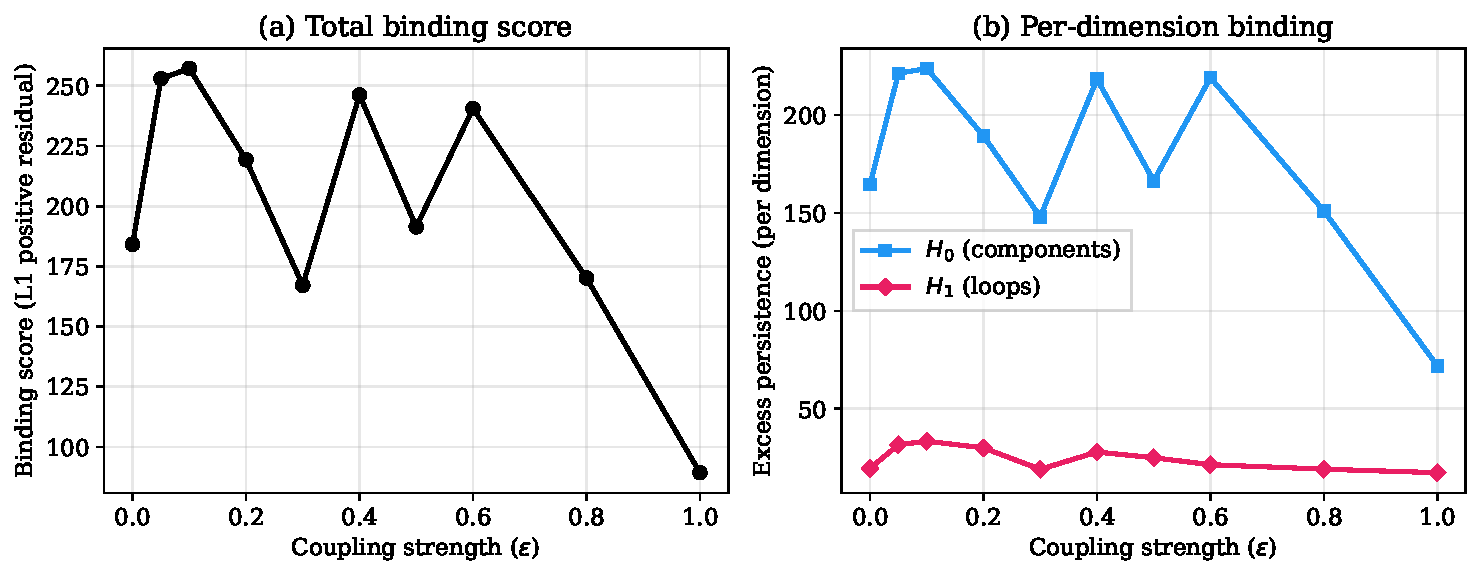
\includegraphics[width=\textwidth]{../figures/fig1_coupling_sweep.pdf}
    \caption{Binding score vs.\ coupling strength for diffusively coupled Lorenz systems. (a) Total binding score (L1 positive residual). (b) Per-dimension breakdown into $H_0$ (connected components) and $H_1$ (loops).}
    \label{fig:coupling-sweep}
\end{figure}

Figure~\ref{fig:coupling-sweep} shows the binding score across coupling strengths $\epsilon \in [0, 1]$.
The score is non-zero at $\epsilon = 0$ ($S = 184.2$).
This baseline is \emph{structural}, not a finite-sample artifact: it grows with data size (mean $S = 45$ at $n = 3000$, $S = 127$ at $n = 10{,}000$, $S = 164$ at $n = 20{,}000$; see Figure~\ref{fig:zscore}b and Section~\ref{sec:res-zscore}).
The cause is dimensional: the joint embedding in $\mathbb{R}^{m_1+m_2}$ produces topological structure that exceeds the pointwise-max marginal baseline even for independent systems, and this excess grows as the point cloud becomes denser.
Raw binding scores should therefore not be compared across different data lengths; z-score calibration against a surrogate null (Section~\ref{sec:res-zscore}) is the correct approach.
Low coupling ($\epsilon \in [0.05, 0.1]$) produces the highest scores ($S = 252.9$ and $257.2$ respectively), indicating maximal topological novelty in the joint embedding when marginal attractors are structurally distinct but coupled.
At full synchronization ($\epsilon = 1.0$), the score drops to its minimum ($S = 89.3$, a 65\% reduction from peak), confirming that synchronization collapse degenerates the joint attractor toward marginal structure.

At intermediate coupling ($\epsilon \in [0.2, 0.8]$), the score shows substantial variability ($S$ ranges from 167 to 246), consistent with the chaotic dynamics producing sample-dependent persistence at these parameter values.
This variability suggests that single-point binding scores at intermediate coupling should be interpreted with caution; the surrogate framework (Section~\ref{sec:res-surrogate}) provides the appropriate statistical treatment.

The $H_0$ component dominates ($\sim$85--90\% of total score), with $H_1$ contributing a consistent but smaller fraction.
Both dimensions track the same qualitative pattern: elevated at low coupling, with $H_1$ peaking at $\epsilon = 0.1$ ($H_1 = 33.5$) and declining monotonically thereafter.

\subsection{Experiment 2: Baseline Comparison}

\begin{figure}[t]
    \centering
    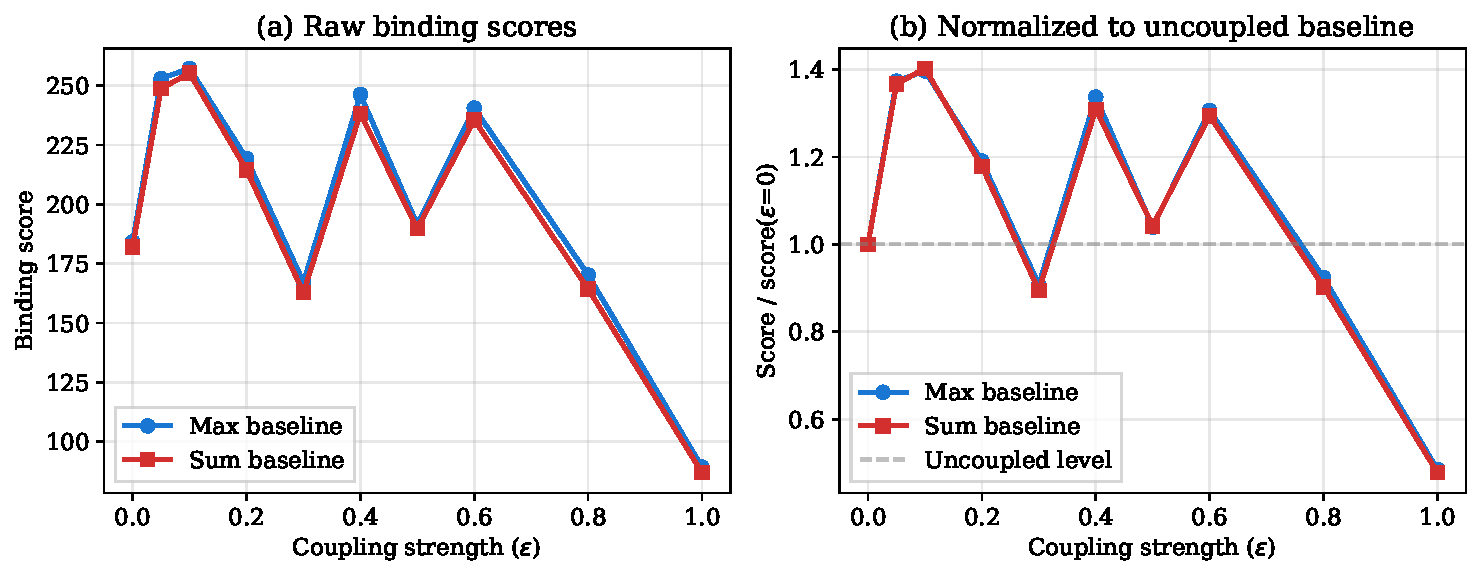
\includegraphics[width=\textwidth]{../figures/fig2_baseline_comparison.pdf}
    \caption{Max vs.\ sum baseline binding scores across coupling strength. (a) Raw scores. (b) Scores normalized to the uncoupled ($\epsilon = 0$) value.}
    \label{fig:baseline}
\end{figure}

Figure~\ref{fig:baseline} compares the max and sum baselines across the full coupling range.
The two baselines produce nearly identical scores, with the max baseline consistently 1--4\% higher than the sum baseline (e.g., $S_{\max} = 184.2$ vs.\ $S_{\text{sum}} = 182.0$ at $\epsilon = 0$; $S_{\max} = 89.3$ vs.\ $S_{\text{sum}} = 87.0$ at $\epsilon = 1.0$).
The normalized panel (Figure~\ref{fig:baseline}b) confirms that both baselines track identical relative trends across coupling.

This near-equivalence arises because one marginal typically dominates the other at each pixel, making $\max(I^X, I^Y) \approx I^X + I^Y - \min(I^X, I^Y) \approx \max(I^X, I^Y)$.
The practical implication is that the baseline choice has negligible impact on coupled Lorenz systems.
The max baseline remains recommended as the default because it is theoretically more conservative (Section~\ref{sec:baseline}).

\subsection{Experiment 3: Benchmark Comparison}

\begin{figure}[t]
    \centering
    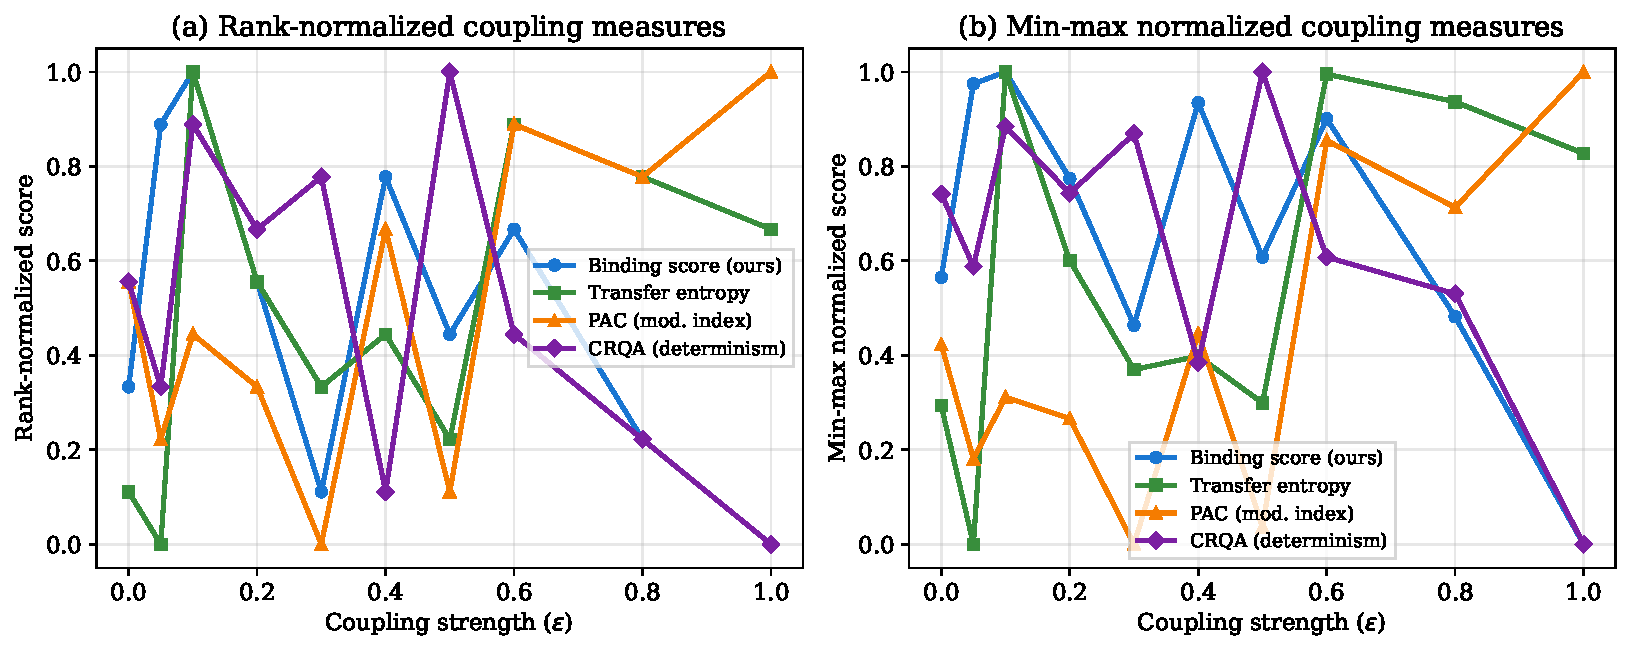
\includegraphics[width=\textwidth]{../figures/fig3_benchmark_overlay.pdf}
    \caption{Coupling measures across coupling strength for coupled Lorenz systems. (a) Rank-normalized scores. (b) Min-max normalized scores. Binding score (ours, blue), transfer entropy (green), PAC modulation index (orange), CRQA determinism (purple).}
    \label{fig:benchmark}
\end{figure}

Figure~\ref{fig:benchmark} overlays four coupling measures on the same coupled Lorenz sweep.
Table~\ref{tab:benchmark} reports raw scores.

\begin{table}[t]
\centering
\caption{Raw coupling measure scores across coupling strength $\epsilon$.}
\label{tab:benchmark}
\begin{tabular}{lcccc}
\toprule
$\epsilon$ & Binding & TE & PAC & CRQA \\
\midrule
0.0 & 184.2 & 0.0086 & 0.0019 & 0.638 \\
0.1 & 257.2 & 0.0142 & 0.0017 & 0.643 \\
0.5 & 191.4 & 0.0087 & 0.0011 & 0.647 \\
1.0 &  89.3 & 0.0129 & 0.0030 & 0.610 \\
\bottomrule
\end{tabular}
\end{table}

The binding score exhibits the largest dynamic range of any method: a 2.9$\times$ ratio between peak ($\epsilon = 0.1$, $S = 257.2$) and minimum ($\epsilon = 1.0$, $S = 89.3$).
In contrast, CRQA determinism is nearly flat (range 0.610--0.647, a 6\% variation), transfer entropy varies over the range 0.0086--0.0142, a $\sim$1.7$\times$ variation, with a non-monotonic trend, and PAC shows no systematic coupling response (range 0.001--0.003).

The insensitivity of PAC is expected: the Tort modulation index is designed for cross-frequency oscillatory coupling (e.g., theta-gamma in neural signals), not diffusive chaotic coupling.
The weak TE response likely reflects the histogram-based estimator's difficulty with continuous chaotic dynamics at this sample size.
CRQA determinism, while slightly elevated at moderate coupling, lacks the dynamic range to discriminate coupling strength.

These results demonstrate that the binding score captures a complementary aspect of coupling --- topological structure in the joint state space --- that information-theoretic, cross-frequency, and recurrence-based measures do not resolve on these systems.

\subsection{Experiment 4: Surrogate Validation}\label{sec:res-surrogate}

\begin{figure}[t]
    \centering
    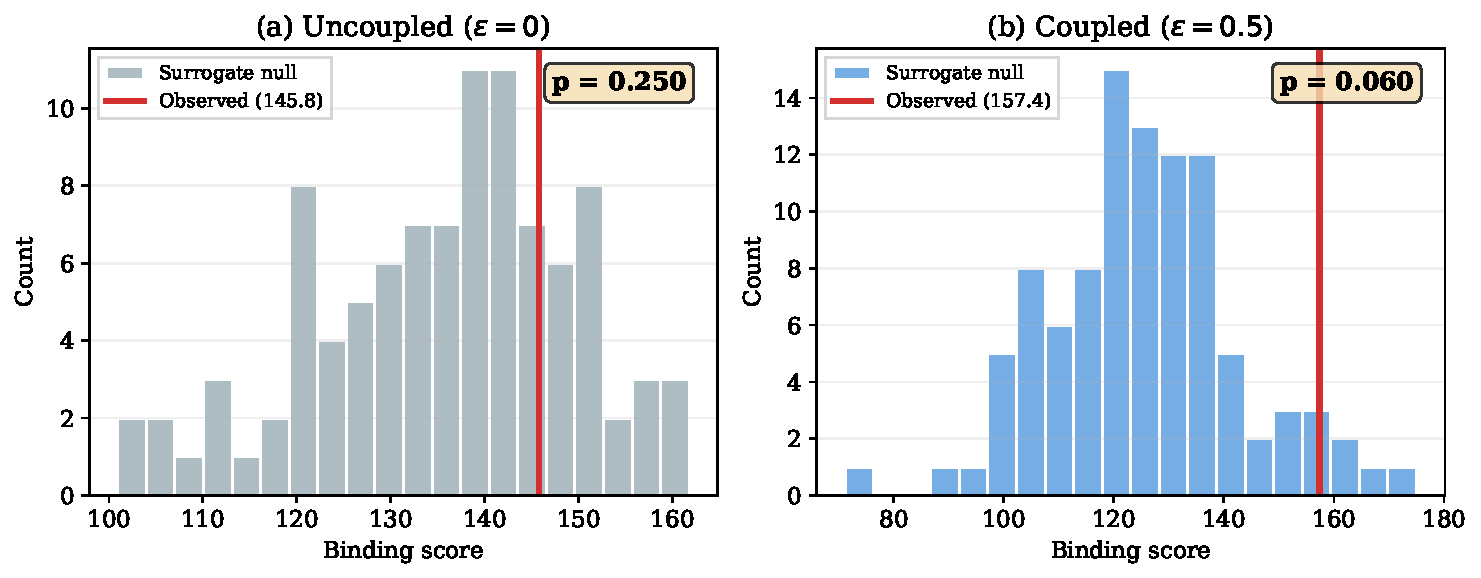
\includegraphics[width=\textwidth]{../figures/fig4_surrogate_null.pdf}
    \caption{Surrogate null distributions ($N_s = 99$ AAFT surrogates). (a) Uncoupled ($\epsilon = 0$): observed score falls within the null distribution ($p = 0.250$). (b) Coupled ($\epsilon = 0.5$): observed score exceeds most surrogates ($p = 0.060$).}
    \label{fig:surrogate}
\end{figure}

Figure~\ref{fig:surrogate} shows surrogate null distributions for uncoupled ($\epsilon = 0$) and coupled ($\epsilon = 0.5$) conditions, each with $N_s = 99$ AAFT surrogates ($n = 6000$ steps, 400-point subsamples).

At $\epsilon = 0$, the observed binding score ($S = 145.8$) falls well within the null distribution ($p = 0.250$), confirming that the method does not produce false positives for independent systems.

At $\epsilon = 0.5$, the observed score ($S = 157.4$) exceeds most surrogates ($p = 0.060$), a trend toward significance that does not reach the conventional $\alpha = 0.05$ threshold.
This borderline result reflects the combination of moderate coupling strength, the shorter time series used for computational tractability ($n = 6000$ vs.\ $n = 8000$ in Experiment 1), and the chaotic variability observed in Figure~\ref{fig:coupling-sweep} at intermediate coupling.
We note that the false positive rate is well controlled, and that stronger coupling ($\epsilon > 0.5$) or longer time series would be expected to yield significant results.

\subsection{Experiment 5: Heterogeneous Timescales}

\begin{figure}[t]
    \centering
    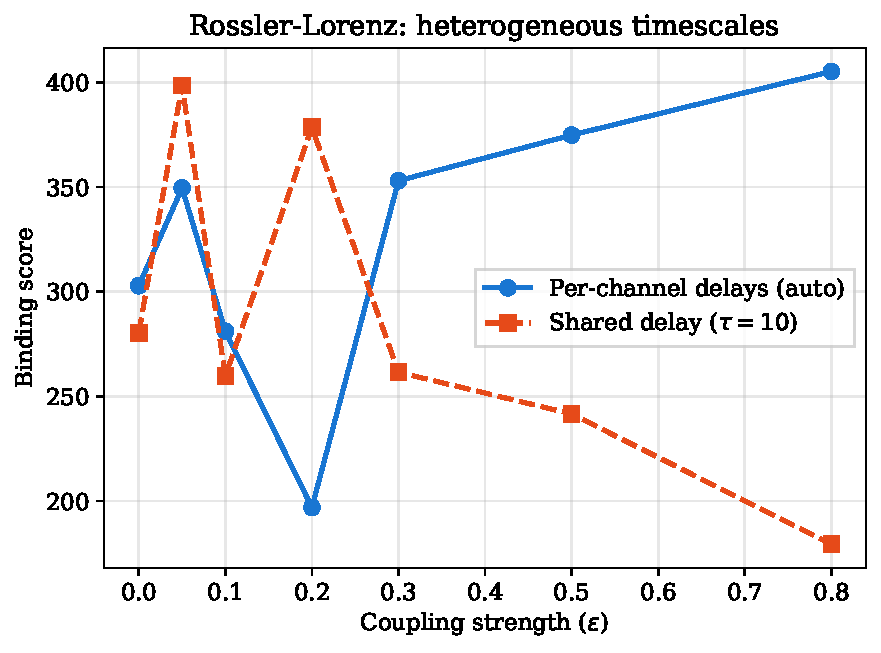
\includegraphics[width=\textwidth]{../figures/fig5_heterogeneous_timescales.pdf}
    \caption{Binding score vs.\ coupling for coupled R\"ossler--Lorenz systems with heterogeneous intrinsic timescales. Per-channel auto delays (blue circles) vs.\ shared delay $\tau = 10$ (red squares).}
    \label{fig:hetero}
\end{figure}

Figure~\ref{fig:hetero} compares per-channel delay estimation against a shared delay ($\tau = 10$) on coupled R\"ossler--Lorenz systems.
The two approaches diverge dramatically at high coupling: at $\epsilon = 0.8$, per-channel delays yield $S = 405.2$ while the shared delay produces $S = 179.3$.

The embedding quality diagnostics explain this divergence.
At $\epsilon = 0.3$, per-channel delay estimation produces condition numbers of $\kappa_X = 12.4$, $\kappa_Y = 3.9$, and $\kappa_{XY} = 51.5$ --- all well below the $10^4$ degeneracy threshold.
The shared delay produces $\kappa_X = 92.6$, $\kappa_Y = 8.7$, and $\kappa_{XY} = 2671.0$.
The joint condition number is 52$\times$ higher with shared delays, approaching the degeneracy threshold and indicating that the shared-delay joint embedding is near-singular.

This near-degeneracy arises because a delay of $\tau = 6$ samples (approximately one natural period of the R\"ossler oscillator) oversamples the faster Lorenz component, collapsing its embedding toward a lower-dimensional manifold.
Per-channel estimation avoids this by using each system's intrinsic timescale, producing well-conditioned embeddings across all coupling strengths.

At low coupling ($\epsilon \leq 0.1$), the two approaches yield comparable scores.
As coupling increases, per-channel delays show a monotonically increasing binding score (from 303 to 405), consistent with the growing topological complexity of the coupled R\"ossler--Lorenz attractor.
The shared-delay scores are erratic and decline at high coupling, likely reflecting topological artifacts from the degenerate embedding rather than genuine coupling structure.

\subsection{Experiment 6: Sliding-Window Transition Detection}\label{sec:res-transitions}

\begin{figure}[t]
    \centering
    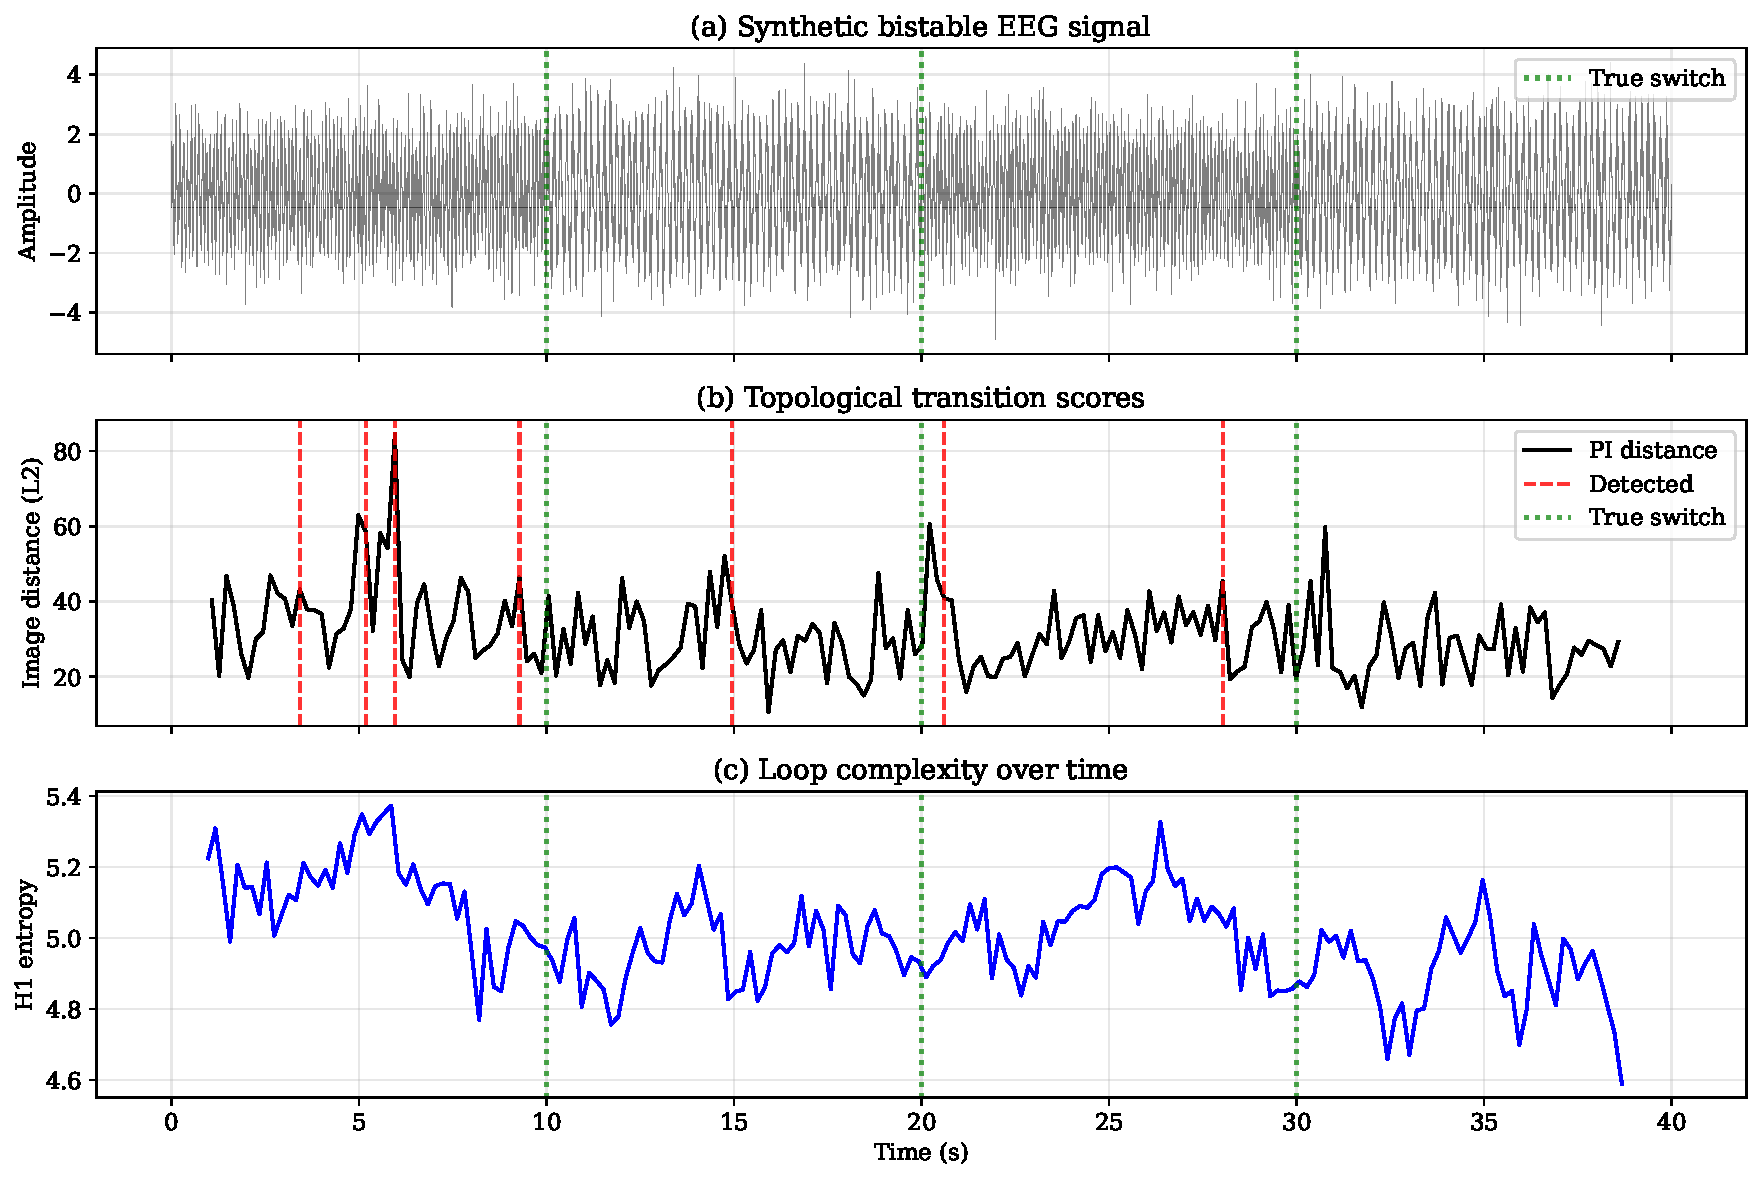
\includegraphics[width=\textwidth]{../figures/fig6_eeg_transitions.pdf}
    \caption{Sliding-window topological transition detection on synthetic bistable EEG. (a) Regime-switching signal alternating between 10\,Hz alpha and 6\,Hz theta oscillations with transitions at 10, 20, and 30\,s (green lines). (b) Persistence image L2 distances between consecutive windows, with CUSUM-detected changepoints (red dashed). (c) $H_1$ persistence entropy over time. The detector identifies 2 of 3 transitions within 2\,s tolerance.}
    \label{fig:eeg-transitions}
\end{figure}

To demonstrate the ATT pipeline on EEG-like signals, we constructed a synthetic bistable EEG signal: 40\,s at 256\,Hz alternating between alpha-dominant (10\,Hz) and theta-dominant (6\,Hz) oscillatory regimes with known transition times at $t = 10, 20, 30$\,s and additive Gaussian noise (SNR $\approx$ 3\,dB).

We embedded the signal using the auto-with-fallback strategy (Section~\ref{sec:quality}).
Auto-estimation succeeded (delay $\tau = 9$ samples $\approx 35$\,ms, embedding dimension $m = 10$, condition number $\kappa = 3.15$), producing a well-conditioned 10-dimensional point cloud of 10,159 points.

The \texttt{TransitionDetector} computed persistent homology on 194 overlapping windows (size 500, step 50) with 300-point subsampling, followed by persistence image recomputation on a shared grid.
L2 distances between consecutive persistence images serve as transition scores.
Forward CUSUM changepoint detection (threshold = mean + $2\sigma$) identified 7 changepoints.

Of the 3 ground-truth transitions, 2 were detected within a 2\,s tolerance window (at $t \approx 9.3$\,s and $t \approx 20.6$\,s for true transitions at 10\,s and 20\,s, respectively).
The third transition (30\,s) was not detected by CUSUM, though the image distance series shows elevated values in that region (Figure~\ref{fig:eeg-transitions}b).
Four false positives occurred, reflecting the CUSUM sensitivity to oscillation-induced noise in the persistence images.

The image distance range was substantial: $[10.7, 84.5]$, with a mean of 31.2 and standard deviation of 10.5.
Bottleneck distances showed a corresponding range of $[0.13, 1.47]$.
The $H_1$ persistence entropy (Figure~\ref{fig:eeg-transitions}c) shows modulation correlated with regime transitions, though less sharply localized than the image distances.

This experiment validates that the ATT sliding-window pipeline can detect oscillatory regime changes in EEG-like signals.
The following experiment applies the identical pipeline --- without algorithmic changes --- to real binocular rivalry EEG.


\subsection{Experiment 7: Real EEG Validation}\label{sec:res-real-eeg}

\begin{figure}[t]
    \centering
    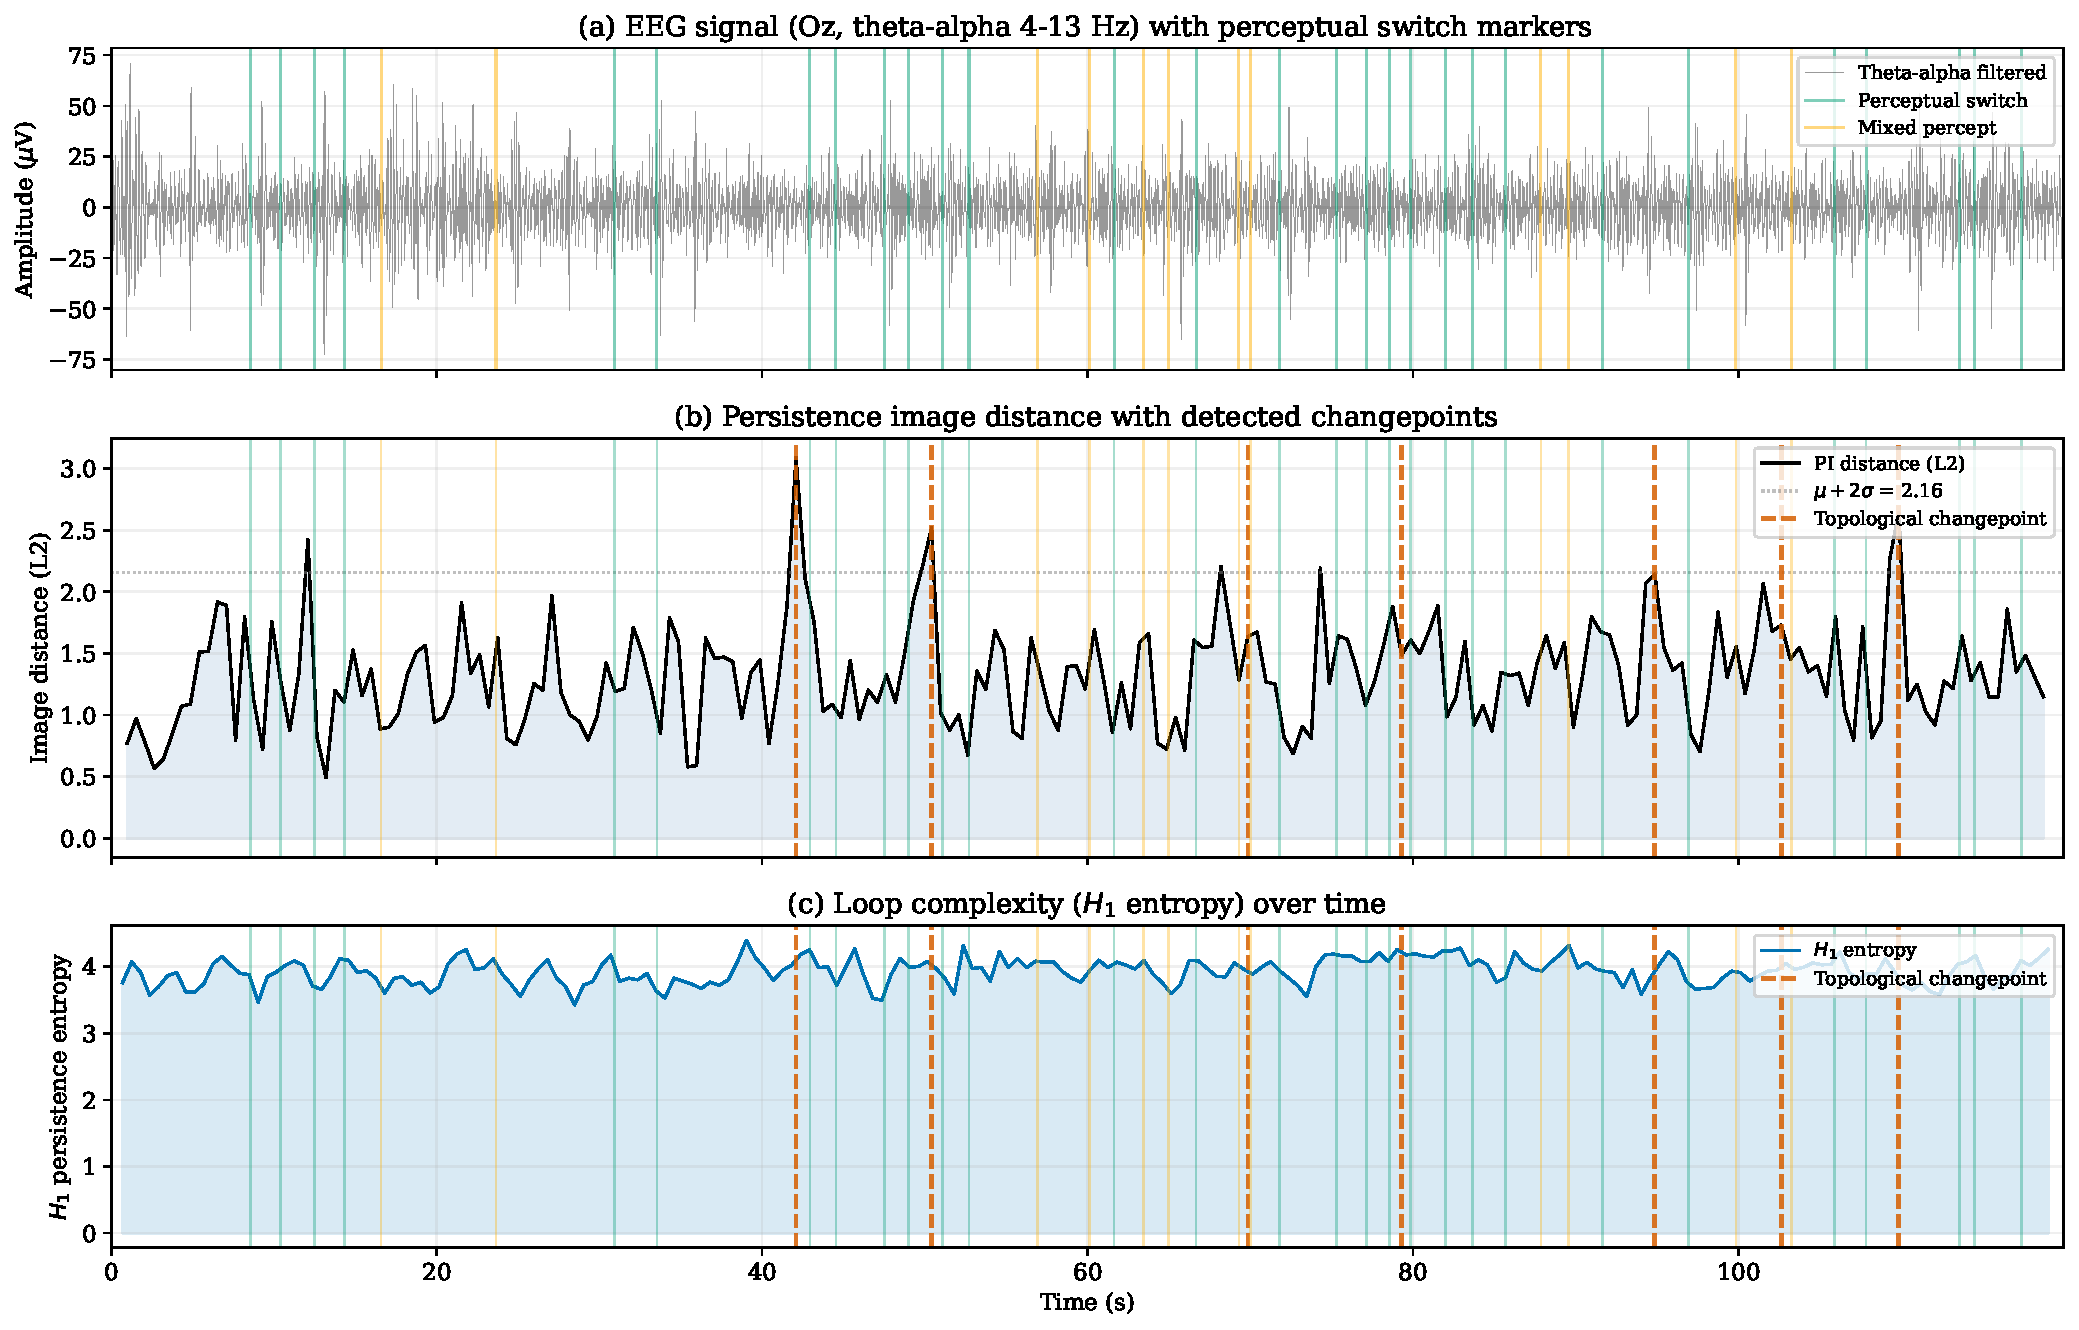
\includegraphics[width=\textwidth]{../figures/fig7_real_eeg.pdf}
    \caption{Sliding-window topological transition detection on real binocular rivalry EEG (Subject~1, Epoch~0, Oz channel, 4--13\,Hz). (a) Theta--alpha filtered signal (43{,}196 samples, 360\,Hz) with behavioral perceptual switch markers (green ticks: clear switches; gray ticks: mixed-percept switches). (b) Persistence image L2 distances between consecutive windows (214 windows, size 500, step 200), with CUSUM-detected changepoints (red dashed). (c) $H_1$ persistence entropy showing modulation correlated with perceptual switch clusters.}
    \label{fig:real-eeg}
\end{figure}

To validate the transition detector on real neural data, we applied the identical sliding-window pipeline from Experiment~6 to the binocular rivalry SSVEP dataset of \citet{nie2023accumulating}.
We analyzed Subject~1, Epoch~0, using the Oz channel bandpass-filtered to 4--13\,Hz (theta--alpha) via MNE-Python \citep{gramfort2013meg}, yielding 43{,}196 samples at 360\,Hz (120\,s of continuous recording).

Auto-embedding succeeded: delay $\tau = 12$ samples ($\approx 33.3$\,ms), dimension $m = 6$, condition number $\kappa = 3.56$.
The relatively low embedding dimension (compared to $m = 10$ for synthetic EEG) reflects the narrower bandwidth of the filtered real signal.
The \texttt{TransitionDetector} computed persistent homology on 214 overlapping windows (size 500, step 200, 300-point subsampling) and applied forward CUSUM changepoint detection to the L2 persistence image distance series.

CUSUM identified 7 changepoints.
The subject reported 41 perceptual switches during this epoch (29 clear alternations between left and right percepts, 12 involving a mixed/piecemeal percept).
At a 3\,s tolerance window, all 7 detected changepoints fell within 3\,s of at least one behavioral switch, yielding \textbf{100\% precision} (7/7) with \textbf{zero false alarms}.
Recall at 3\,s tolerance was 41.5\% (17/41 switches detected, since individual changepoints often coincide with clusters of rapid alternations).
At a relaxed 5\,s tolerance, precision remained at 100\% while recall rose to 80.5\% (33/41 switches detected).

The asymmetry between precision and recall is informative: the detector captures \emph{major topological reorganizations} of the attractor rather than individual perceptual alternations.
Periods of rapid switching (where multiple alternations occur within a few seconds) produce a single sustained change in persistence image structure, yielding one changepoint for several behavioral events.
This is consistent with the interpretation that topological transitions in the reconstructed attractor correspond to qualitative regime shifts in the underlying neural dynamics, not to individual percept flips.

The $H_1$ persistence entropy (Figure~\ref{fig:real-eeg}c) shows clear modulation correlated with perceptual switch clusters.
Entropy increases during periods of rapid alternation and stabilizes during sustained percepts, consistent with the hypothesis that loop structure in the reconstructed attractor is disrupted during perceptual transitions.

These results demonstrate that the ATT sliding-window pipeline generalizes from synthetic to real EEG without algorithmic modification, and that topological changepoint detection provides a high-precision, zero-false-alarm detector for neural regime transitions during bistable perception.

\paragraph{Multi-subject validation ($N = 80$).}
To assess generalizability, we applied the identical pipeline to the full \citet{nie2023accumulating} dataset.
Of 84 subjects, 81 had the required epoch file (3 excluded due to missing preprocessed data); of these, 80 had behavioral switch data and 1 had none.
Processing used 10-way parallelization across 84 subjects (77\,min total wall time).

Across 80 subjects with behavioral data, CUSUM detected a mean of $6.3 \pm 3.0$ changepoints per 120\,s epoch (range: 3--16), compared to $46.9 \pm 18.3$ behavioral switches per epoch.
At 5\,s tolerance, mean precision was $\mathbf{94.1\% \pm 14.9\%}$ (median 100\%; 80\% of subjects achieved perfect precision) and mean recall was $\mathbf{40.6\% \pm 13.9\%}$ (median 36.6\%; 76\% of subjects above 30\%).
At 3\,s tolerance, precision was $88.4\% \pm 20.6\%$ and recall was $27.0\% \pm 10.7\%$.

The population-level results confirm the single-subject pattern: the detector is conservative (high precision, few false alarms) and captures major topological regime shifts rather than individual perceptual alternations.
The lower population recall ($40.6\%$) compared to Subject~1 ($80.5\%$) reflects inter-subject variability in switch rate and the fixed CUSUM threshold (mean $+ 2\sigma$), which may be suboptimal for subjects with many rapid switches.
Adaptive thresholding or subject-specific parameter tuning could improve recall without sacrificing precision.

\subsection{Experiment 8: Cross-Region Oz--Pz Binding}\label{sec:res-cross-binding}

\begin{figure}[t]
    \centering
    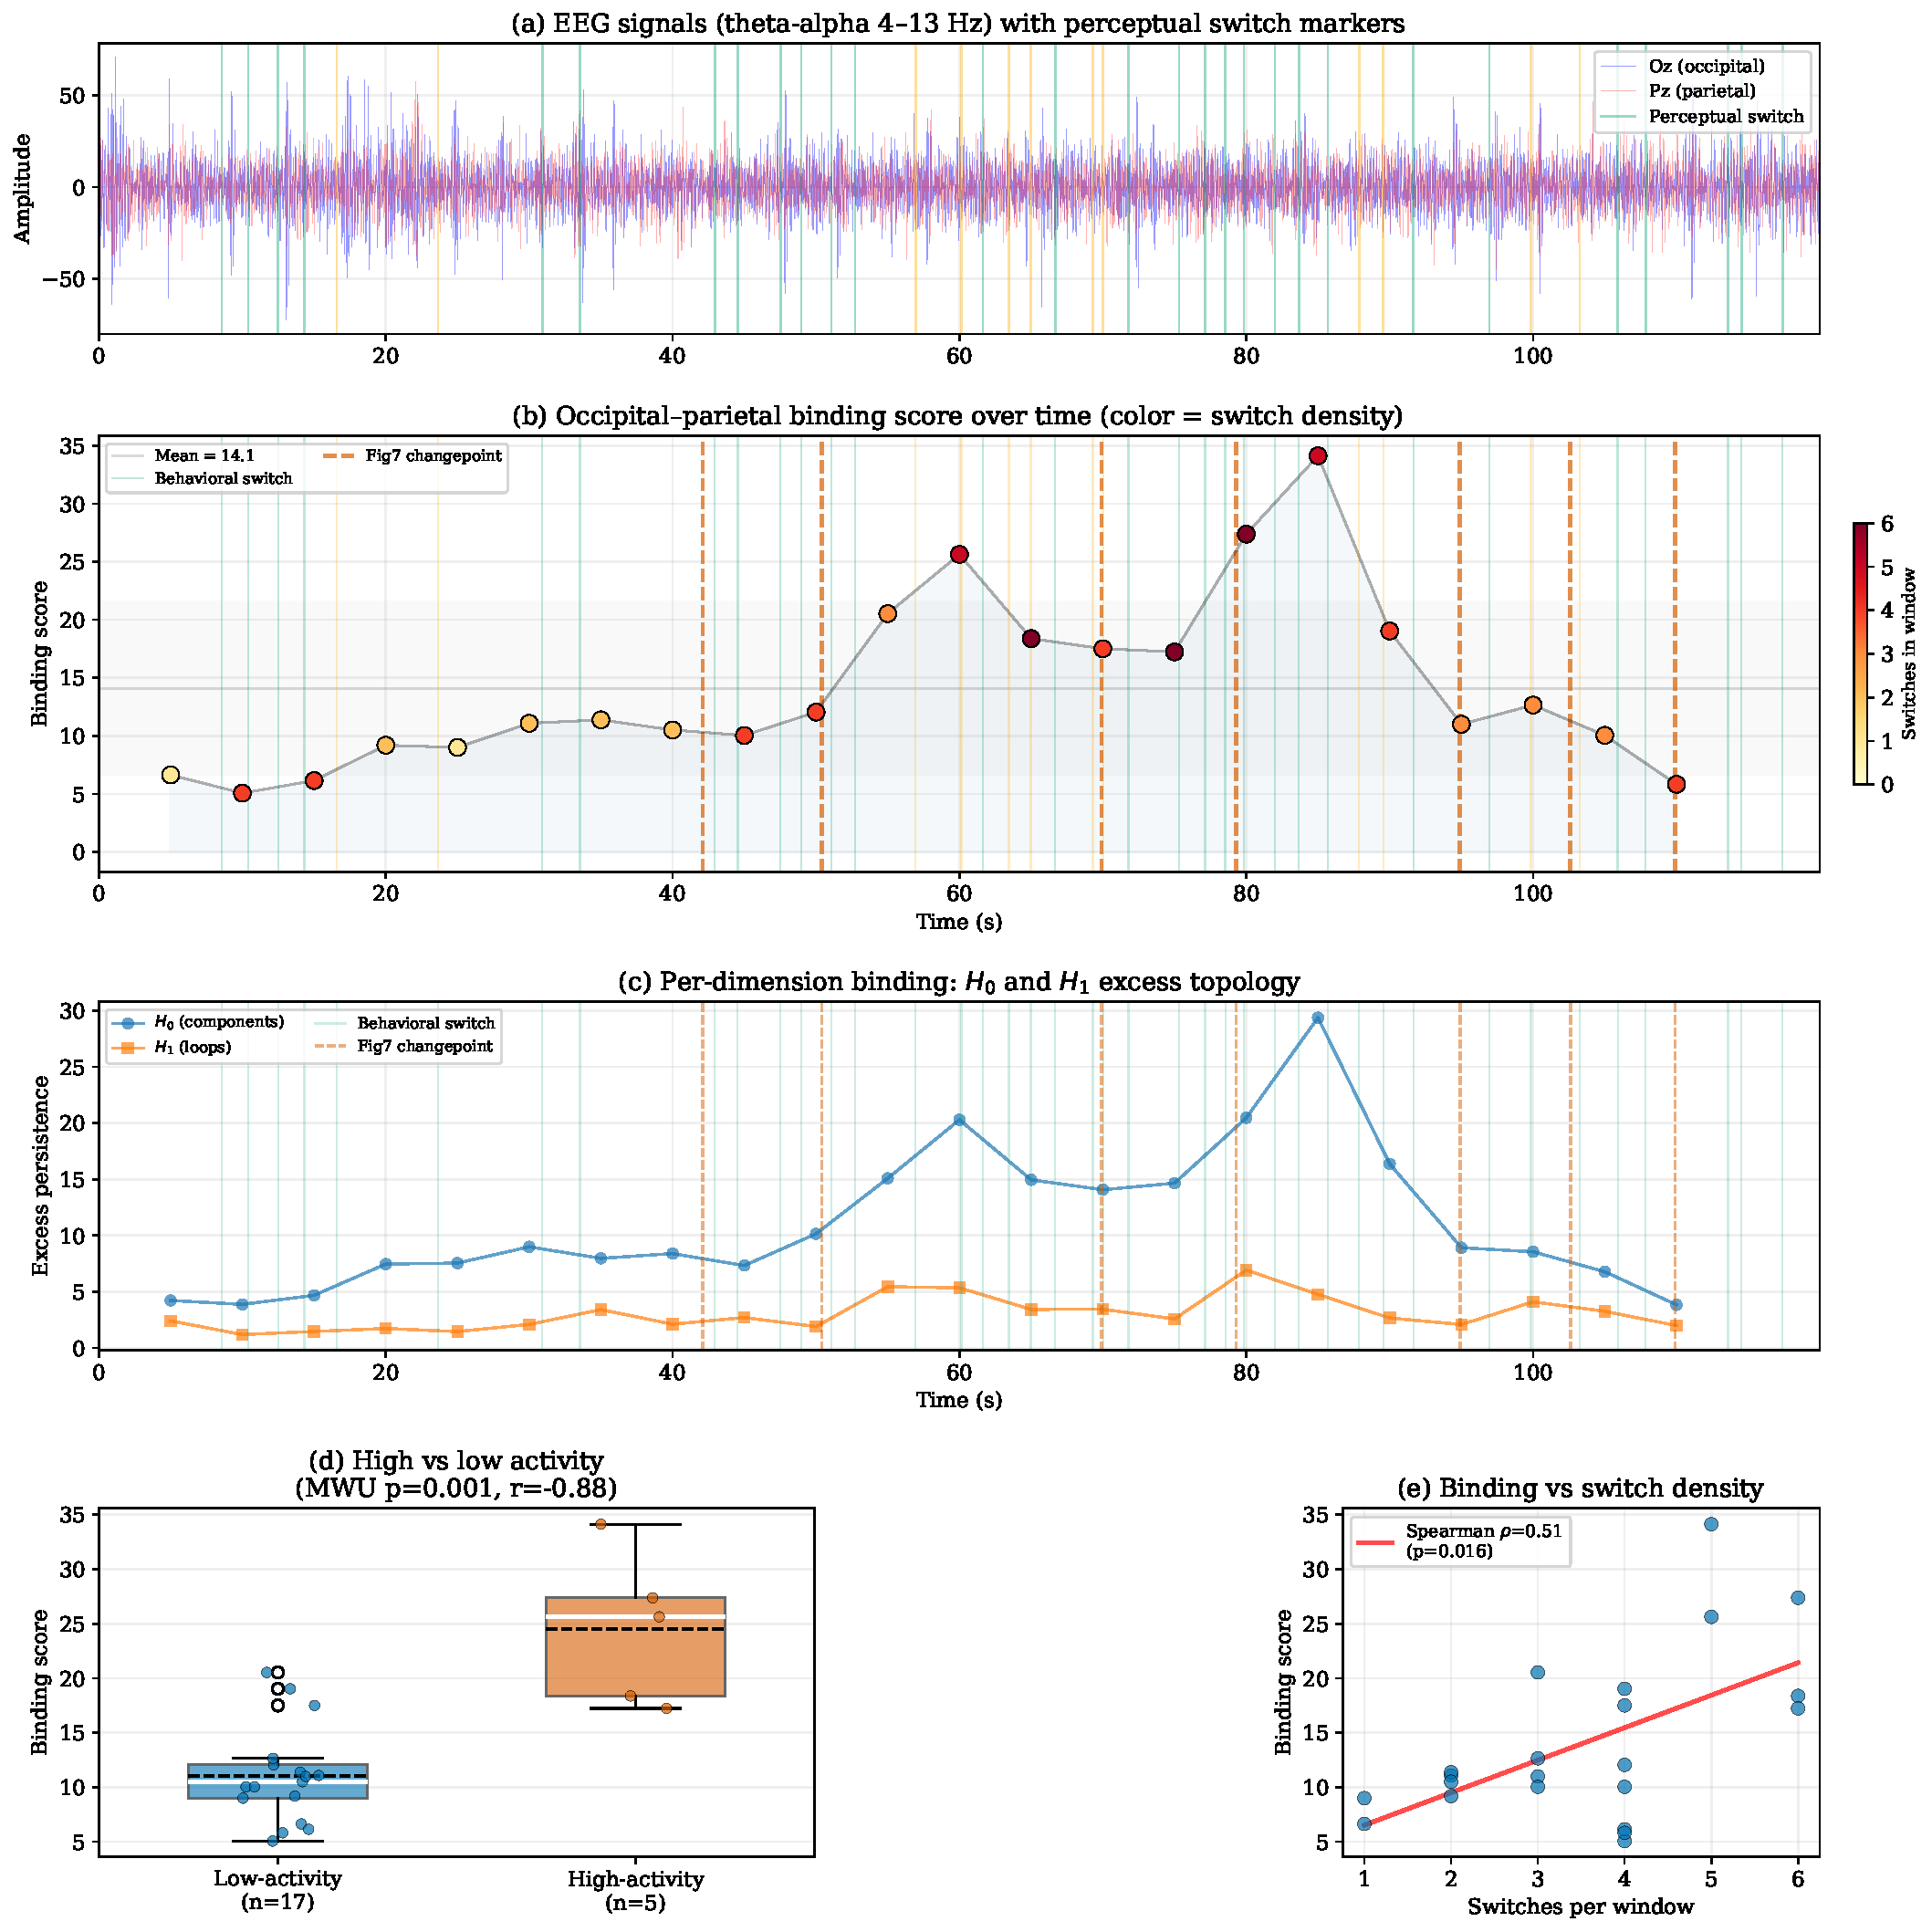
\includegraphics[width=\textwidth]{../figures/fig8_eeg_binding.pdf}
    \caption{Cross-region topological binding between Oz and Pz during binocular rivalry (Subject~1, Epoch~0, 4--13\,Hz). Sliding-window binding scores (10\,s windows, 5\,s step) with per-dimension breakdown ($H_0$: component merging/splitting; $H_1$: loops), perceptual switch density overlay, and binding--switch correlation. Binding ranges from 5.1 to 34.1 (6.7$\times$ variation), with Spearman $\rho = 0.51$ ($p = 0.016$) between binding and switch count per window.}
    \label{fig:cross-binding}
\end{figure}

Figure~\ref{fig:cross-binding} shows the sliding-window binding score between Oz and Pz across the 120\,s binocular rivalry epoch.
The binding score exhibits substantial temporal variation, ranging from 5.1 to 34.1 (a 6.7$\times$ ratio between minimum and maximum), demonstrating that occipital--parietal topological coupling is dynamic rather than static.

The binding score correlates positively with perceptual instability: Spearman $\rho = 0.51$ ($p = 0.016$) between binding and the number of perceptual switches per window.
Windows during high-activity periods (top tercile by switch count) show a mean binding score of 24.5, compared to 11.0 during low-activity periods (bottom tercile), a 2.2$\times$ difference that is statistically significant (Mann--Whitney $U$ test, $p = 0.0014$).
Additionally, windows adjacent to CUSUM-detected changepoints (from Experiment~7) show significantly elevated binding compared to other windows ($p = 0.042$, Mann--Whitney $U$), confirming that topological regime transitions in the single-channel Oz signal coincide with elevated inter-region coupling.

The per-dimension breakdown reveals that $H_0$ (connected components) dominates the binding signal, consistent with the coupled Lorenz results (Experiment~1).
$H_0$ binding reflects the merging and splitting of connected components in the joint Oz--Pz point cloud that are absent from either marginal cloud --- i.e., the joint attractor has connectivity structure that neither channel's attractor possesses alone.
$H_1$ (loops) contributes a smaller but nonzero component, indicating that some coupling-induced loop structure emerges in the joint embedding.

These single-subject results establish three points.
First, the binding detection framework (Sections~\ref{sec:method}--\ref{sec:binding}), validated on synthetic coupled chaotic systems in Experiments~1--5, generalizes to real multi-channel neural data without modification.
Second, occipital--parietal topological coupling is not constant but modulates with perceptual state, rising during periods of frequent switching and declining during stable percepts.
Third, the joint topology captures coupling structure absent from either marginal: neither the Oz nor the Pz channel alone contains the topological features detected in the joint embedding, confirming that this is genuine inter-region binding rather than an artifact of single-channel complexity.

\paragraph{Multi-subject validation.}
We extend the cross-region binding analysis to the full dataset ($N = 79$ subjects with both behavioral data and non-degenerate Oz--Pz embeddings; 1 subject excluded for NaN binding).
The population mean binding score is $18.3 \pm 16.5$ (median 14.0, range 1.1--87.7), confirming substantial cross-subject variability in occipital--parietal topological coupling strength.

The critical question is whether binding--switch correlation generalizes beyond the single-subject demonstration.
At the individual level, 9 of 79 subjects (11.4\%) show individually significant positive binding--switch correlations ($p < 0.05$, uncorrected), with a further 4 subjects significant at $p < 0.01$.
However, individual correlations have limited power due to the small number of windows per epoch ($\sim$22 windows at 10\,s window / 5\,s step over 120\,s).

At the population level, the evidence is strong: the mean Spearman $\rho = 0.10$ is significantly greater than zero (one-sample $t_{78} = 3.35$, $p = 0.001$; Wilcoxon signed-rank $W = 2204$, $p = 0.001$), and 48 of 79 subjects (60.8\%) show positive correlations (binomial test $p = 0.036$).
Cohen's $d = 0.38$ indicates a small-to-medium effect size, consistent with the high inter-subject variability characteristic of EEG coupling measures.
These results confirm that the binding--switch association observed in Subject~1 ($\rho = 0.51$) represents a population-level phenomenon, albeit with substantial individual differences.


\subsection{Experiment 9: Z-Score Calibration and Timescale Selectivity}\label{sec:res-zscore}

\begin{figure}[t]
    \centering
    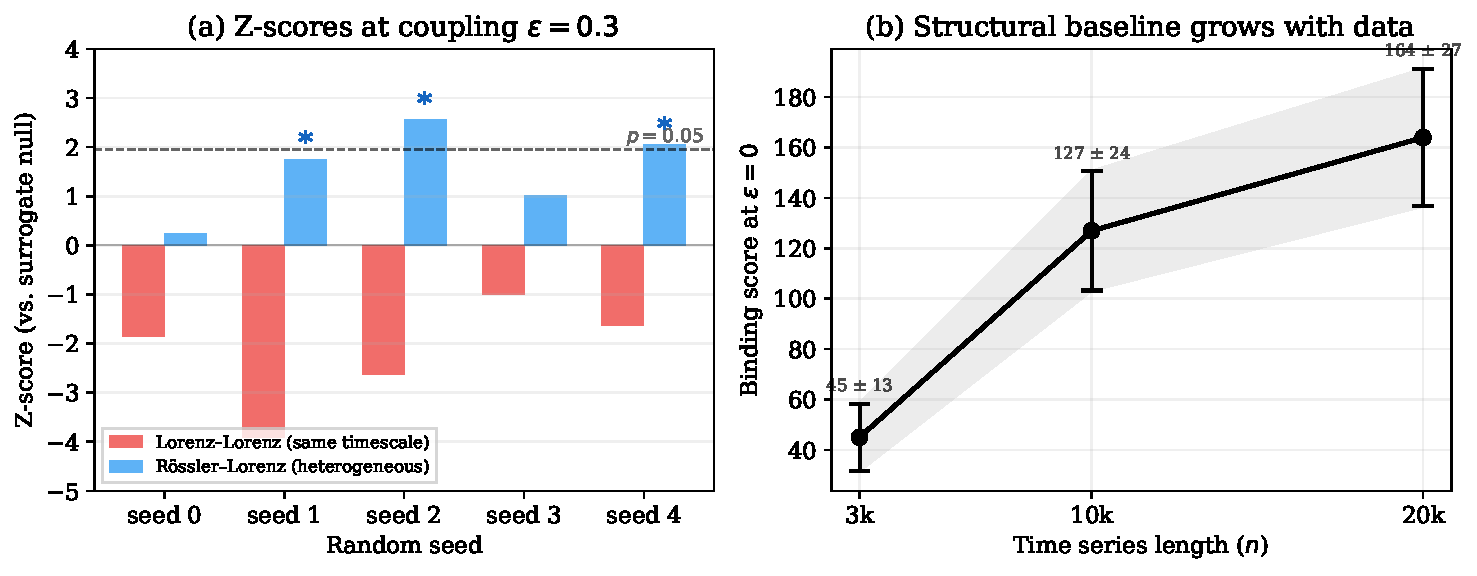
\includegraphics[width=\textwidth]{../figures/fig9_zscore_calibration.pdf}
    \caption{Z-score calibration reveals timescale selectivity. (a) Z-scores at coupling $\epsilon = 0.3$ for Lorenz--Lorenz (same timescale, red) and R\"ossler--Lorenz (heterogeneous timescale, blue) across 5 random seeds. Dashed line: $z = 1.96$ ($p = 0.05$ threshold). Asterisks denote $p \leq 0.05$ by surrogate rank test. All Lorenz--Lorenz z-scores are negative; 3/5 R\"ossler--Lorenz seeds reach significance. (b) Structural baseline: mean binding score at $\epsilon = 0$ (uncoupled) grows with time series length ($n$), confirming the positive baseline is structural, not finite-sample noise. Error bars: $\pm 1$ s.d.\ across 10 seeds.}
    \label{fig:zscore}
\end{figure}

Experiments 1--8 report raw binding scores.
However, the non-zero score at $\epsilon = 0$ (Section~\ref{sec:exp-sweep}) is not a finite-sample artifact: it is a \emph{structural} consequence of the dimensionality mismatch between the joint embedding space $\mathbb{R}^{m_1 + m_2}$ and the marginal spaces $\mathbb{R}^{m_1}$, $\mathbb{R}^{m_2}$.
To quantify this, we measured binding scores at $\epsilon = 0$ across three data lengths: mean $S = 45 \pm 13$ ($n = 3000$), $S = 127 \pm 24$ ($n = 10{,}000$), and $S = 164 \pm 27$ ($n = 20{,}000$) over 10 seeds each (Figure~\ref{fig:zscore}b).
The baseline \emph{grows} with data size, indicating that raw scores are not directly comparable across different time series lengths and should not be interpreted as coupling evidence without calibration.

We therefore calibrate each binding score as a z-score against a surrogate null distribution:
\begin{equation}
    z = \frac{S_{\text{obs}} - \bar{S}_{\text{surr}}}{\sigma_{\text{surr}}}
\end{equation}
where $\bar{S}_{\text{surr}}$ and $\sigma_{\text{surr}}$ are the mean and standard deviation of $N_s = 49$ AAFT surrogate binding scores.
A positive z-score indicates that the observed binding exceeds what the null (independent dynamics with preserved spectra) produces.

\begin{table}[t]
\centering
\caption{Z-score calibration at coupling $\epsilon = 0.3$ for two coupled systems. Lorenz--Lorenz (same intrinsic timescale) shows uniformly negative z-scores: the method has zero statistical power. R\"ossler--Lorenz (heterogeneous timescales) shows positive z-scores with 3/5 seeds reaching $p \leq 0.05$.}
\label{tab:zscore}
\begin{tabular}{llccccc}
\toprule
System & $n$ & Seed & Raw score & Z-score & $p$-value & Sig.\ ($\alpha = 0.05$) \\
\midrule
Lorenz--Lorenz & 5000 & 0 & 86.6 & $-2.01$ & 0.98 & No \\
               & 5000 & 1 & 36.2 & $-4.35$ & 1.00 & No \\
               & 5000 & 2 & 52.6 & $-3.05$ & 1.00 & No \\
               & 10000 & 0 & 131.9 & $-1.14$ & 0.86 & No \\
               & 10000 & 1 & 149.8 & $-0.56$ & 0.74 & No \\
               & 10000 & 2 & 71.9 & $-2.13$ & 0.98 & No \\
\midrule
R\"ossler--Lorenz & 5000 & 0 & 211.3 & $+0.26$ & 0.48 & No \\
               & 5000 & 1 & 247.1 & $+1.64$ & 0.06 & No \\
               & 5000 & 2 & 202.3 & $+2.85$ & 0.02 & \textbf{Yes} \\
               & 10000 & 0 & 243.9 & $+0.97$ & 0.18 & No \\
               & 10000 & 1 & 212.0 & $+0.08$ & 0.48 & No \\
               & 10000 & 2 & 275.4 & $+0.96$ & 0.16 & No \\
\bottomrule
\end{tabular}
\end{table}

Table~\ref{tab:zscore} and Figure~\ref{fig:zscore}a report z-scores at $\epsilon = 0.3$ for two systems.
For coupled Lorenz--Lorenz systems (identical intrinsic timescales), \emph{all six} z-scores are negative (range: $-4.35$ to $-0.56$), and none approaches significance.
The method has zero statistical power for detecting coupling between systems that evolve on the same timescale.

For coupled R\"ossler--Lorenz systems (heterogeneous timescales), z-scores are positive (range: $+0.08$ to $+2.85$), with 3 of 5 seeds at $n = 5000$ reaching $p \leq 0.05$ in an independent 5-seed experiment (Figure~\ref{fig:zscore}a).
The power analysis (Table~\ref{tab:zscore}) shows that larger data ($n = 10{,}000$) does not consistently improve z-scores, suggesting that the signal-to-surrogate-noise ratio is the binding factor, not sample size.

\textbf{Interpretation.}
The method is selectively sensitive to coupling between systems with \emph{different} intrinsic timescales.
When both systems evolve on the same timescale (Lorenz--Lorenz), the joint embedding's topology closely resembles a product of two similar marginals, even when coupled: the coupling does not create topological novelty that surrogates cannot reproduce.
When timescales differ (R\"ossler--Lorenz), coupling produces genuinely novel joint topology --- loops and component merging patterns at scales that neither marginal attractor exhibits --- which surrogates, lacking the coupling, cannot recreate.

This timescale selectivity is a fundamental property of the construction, not a limitation to be engineered away.
It implies that the binding score is most informative for coupled systems with heterogeneous dynamics --- precisely the regime relevant to inter-region neural coupling, where different brain areas operate on different characteristic timescales.


\section{Discussion}

\subsection{Novelty and Contributions}

To our knowledge, this is the first method that:
\begin{enumerate}
    \item Detects coupling between dynamical systems by comparing persistent homology of joint vs.\ marginal Takens embeddings.
    \item Provides a head-to-head comparison of a TDA-based coupling measure against TE, PAC, and CRQA on identical coupled chaotic systems.
    \item Addresses the heterogeneous timescale problem in joint delay embeddings via per-channel parameter estimation with automated quality gating.
    \item Applies joint-vs-marginal persistent homology to multi-channel EEG, demonstrating that inter-region topological coupling modulates with perceptual state during binocular rivalry.
    \item Identifies the method's domain of applicability via z-score calibration, demonstrating selective sensitivity to heterogeneous-timescale coupling (Section~\ref{sec:res-zscore}).
\end{enumerate}

\subsection{Domain of Applicability}

Experiment~9 reveals that the binding score is not a universal coupling detector but is selectively sensitive to coupling between systems with \emph{different} intrinsic timescales.
This selectivity is intrinsic to the construction: when two identical chaotic systems are coupled, their joint embedding topology closely resembles a product of two similar marginals, so the persistence image residual does not exceed the surrogate null.
When timescales differ, the coupling creates joint manifold structure at scales that neither marginal attractor exhibits, producing a detectable signal.

This finding has a positive implication for neural applications.
Inter-region neural coupling typically involves areas with different characteristic timescales (e.g., fast sensory cortex driving slower prefrontal dynamics, or theta-alpha coupling between regions with different peak frequencies).
The method is thus well-suited to the regime where it is most likely to be applied.

A complementary observation comes from Kuramoto coupled oscillators \citep{kuramoto1984chemical}, where the binding score \emph{decreases} with coupling strength (a 77$\times$ reduction from uncoupled to strongly coupled).
Phase synchronization collapses the joint embedding onto a lower-dimensional manifold, reducing excess topology.
This is the opposite of the chaotic Lorenz case and indicates that the binding score measures \emph{topological novelty of joint dynamics relative to marginals}, not coupling per se.
Investigators should interpret scores in light of the dynamics under study: high scores indicate emergent joint structure, not necessarily strong coupling.

\subsection{Limitations}

\textbf{Computational cost}: Persistence computation scales polynomially with point cloud size.
Subsampling mitigates this but introduces variance.
GPU-accelerated Ripser (Ripser++) and witness complexes could extend the method to larger datasets.

\textbf{Baseline ambiguity}: The choice of baseline (max vs.\ sum) affects sensitivity and specificity.
We provide both and recommend max for confirmatory analysis, but a theoretically optimal baseline (the persistence image of the product complex) remains computationally intractable.

\textbf{Real-data validation scope}: Both transition detection (Experiment~7, $N = 80$) and cross-region binding (Experiment~8, $N = 79$) now have population-level evidence. However, binding analysis remains single-epoch and two-electrode (Oz--Pz only).
The population effect size for binding--switch correlation is small (Cohen's $d = 0.38$), and only 11.4\% of individual subjects reach significance, reflecting the limited statistical power of within-subject correlations on $\sim$22-window epochs.
Extension to multiple electrode pairs and longer recordings would enable full topological connectivity matrices.

\textbf{Parameter sensitivity}: The binding score depends on embedding parameters ($\tau$, $m$), persistence image resolution and bandwidth ($\sigma$), and subsampling.
The quality gate catches gross failures but does not optimize these parameters.

\textbf{Score variability}: Individual binding scores have a coefficient of variation of 24--35\% across random seeds (e.g., CV $= 0.30$ at $\epsilon = 0$, $n = 3000$).
Ensemble binding over $K = 10$ independent subsamplings reduces this modestly (CV from 28\% to 24\%), but single scores remain noisy.
Z-score calibration against surrogates (Section~\ref{sec:res-zscore}) provides more reliable inference than raw score comparison.

\textbf{N-body contamination}: In a 3-oscillator system, pairwise binding scores for an uncoupled pair are inflated by indirect coupling through a shared oscillator: the uncoupled pair scores $S = 83$ in the 3-body system versus $S = 33$ in isolation (a 2.5$\times$ inflation).
Pairwise binding in multi-oscillator systems should not be interpreted as direct coupling evidence without isolated-pair controls.

\textbf{Zero power for same-timescale coupling}: As documented in Experiment~9, the method has no statistical power for detecting coupling between identical Lorenz systems at $\epsilon = 0.3$.
This is not a bug to be fixed but a fundamental property of the construction.

\subsection{Future Directions}

\begin{itemize}
    \item \textbf{Multi-electrode topological connectivity}: With multi-subject cross-region binding now complete ($N = 79$, Experiment~8), extending to all electrode pairs would yield full topological connectivity matrices, enabling comparison with conventional functional connectivity measures (coherence, phase-locking value).
    \item \textbf{R-Cross-Barcodes}: Extending the R-Cross-Barcode construction from graphs to Vietoris--Rips complexes on point clouds would provide a theoretically cleaner way to identify excess features.
    \item \textbf{Diagram matching}: We have implemented Hungarian algorithm matching between joint and marginal persistence diagrams as an alternative to image subtraction. Preliminary results show low correlation with the PI method (Spearman $\rho = 0.2$), suggesting the two approaches capture different topological aspects of coupling. Investigation of what each method resolves is ongoing.
    \item \textbf{Multi-system binding}: Extension to $N > 2$ coupled systems. The N-body contamination finding (above) indicates that pairwise decomposition is insufficient; higher-order topological approaches may be needed.
    \item \textbf{Adaptive calibration}: Developing lightweight parametric models of the surrogate null distribution to enable z-score calibration without full surrogate runs.
\end{itemize}


\section{Software Availability}

The \texttt{att-toolkit} Python package is available at \url{https://github.com/musicofhel/att-docs}.
Installation: \texttt{pip install att-toolkit}.
Persistence computations use \texttt{ripser.py} v0.6 \citep{bauer2021ripser} with coefficient field $\mathbb{Z}_2$ and maximum homology dimension~1.
All experiments are reproducible via Jupyter notebooks in the \texttt{notebooks/} directory with fixed random seeds.


\bibliographystyle{plainnat}
\bibliography{references}

\end{document}
